\begin{figure}[t]
  \newlength{\figwidth}
  \setlength{\unitlength}{\columnwidth}
  \setlength{\figwidth}{0.8\unitlength}
  \centering
  \subfloat[An \(n \by n\) unitary, implemented in linear optics.]{
    \begin{picture}(1,0.45)
      %\put(0,0){\line(1,0){1}}
      %\put(0,0){\line(0,1){0.45}}
      %\put(0,0.45){\line(1,0){1}}
      %\put(1,0){\line(0,1){0.45}}
      \put(0.15,0){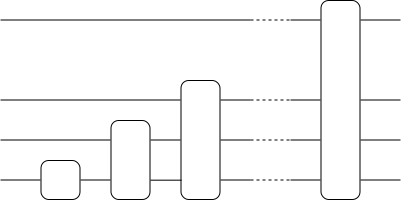
\includegraphics[width=\figwidth]{figures/reck_nxn}}
      % Mode labels
      \put(0.03,0.03){\( n-1 \)}
      \put(0.03,0.11){\( n-2 \)}
      \put(0.03,0.19){\( n-3 \)}
      \put(0.10,0.35){\( 0 \)}
      % Unitary labels
      \put(0.24,0.03){\( R_{1} \)}
      \put(0.38,0.07){\( R_{2} \)}
      \put(0.53,0.11){\( R_{3} \)}
      \put(0.81,0.19){\( R_{n} \)}
    \end{picture}
    \label{fig:recknxn}
  } \\
  \subfloat[The relationship between the \( \vec{x} \) and \( \vec{r} \)
    bases; linear-optical circuit corresponding to the block \(R_{n}\).]{
    \begin{picture}(1.0,0.45)
      %\put(0,0){\line(1,0){1}}
      %\put(0,0){\line(0,1){0.45}}
      %\put(0,0.45){\line(1,0){1}}
      %\put(1,0){\line(0,1){0.45}}
      \put(0.1,0.03){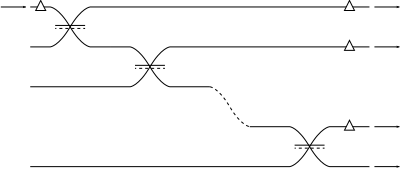
\includegraphics[width=\figwidth]{figures/cascade}}
      %%% x labels
      \put(0.88,0.38){\(x_{0}\)}
      \put(0.88,0.30){\(x_{1}\)}
      \put(0.88,0.14){\(x_{n-2}\)}
      \put(0.88,0.07){\(x_{n-1}\)}
      %%% r labels
      \put(0.10,0.38){\(r_{0}\)}
      \put(0.23,0.38){\(r_{1}\)}
      \put(0.38,0.30){\(r_{2}\)}
      \put(0.68,0.14){\(r_{n-1}\)}
    \end{picture}
    \label{fig:cascade}
  }
  \caption{In~\ref{fig:cascade},
    \(r_{0}\) corresponds to the power of the input light and \(x_{i}\) is the
    power output in mode \(i\). The other \(r\)s correspond to the
    reflectivities of beamsplitters in the circuit. The triangles are phase
    shifts, and may be chosen uniformly from the interval \( \left[ 0, 2\pi
    \right)\), since the phases do not appear in the pdf in either the \(
    \vec{x} \) or the \( \vec{r} \) basis. The unitary describing this set of
    optical components is the matrix \( \mat{R}_{n} \).
    Each of the labelled blocks in~\ref{fig:recknxn} are cascaded beamsplitters
    as illustrated in~\ref{fig:cascade}, and implement the rotation matrices,
    \(\mat{R}_{i}\).}
  \label{fig:reck}
\end{figure}
